\begin{center}
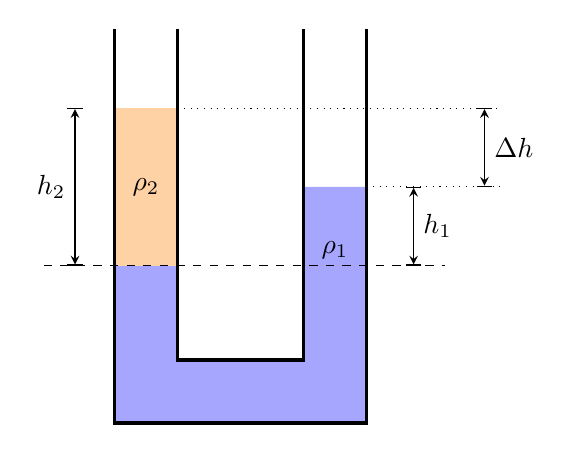
\begin{tikzpicture}[>=stealth]
 \fill[blue!35] (0,0) -- (0,2) -- (0.8,2) -- (0.8,0.8) -- (2.4,0.8) -- (2.4,3) -- (3.2,3) -- (3.2,0) -- cycle;
 \fill[orange!35] (0,2) rectangle (0.8,4);
 \draw[very thick] (0,5) -- (0,0) -- (3.2,0) -- (3.2,5);
 \draw[very thick] (0.8,5) -- (0.8,0.8) -- (2.4,0.8) -- (2.4,5);
 \node at (0.4,3) {$\rho_2$};
 \node at (2.8,2.2) {$\rho_1$};
 \draw[dashed] (-0.9,2) -- (4.2,2);
 \draw[dotted] (0.8,4) -- (4.9,4);
 \draw[dotted] (3.2,3) -- (4.9,3);
 \draw[|<->|] (-0.5,2) -- (-0.5,4) node[midway, left] {$h_2$};
 \draw[|<->|] (3.8,2) -- (3.8,3) node[midway, right] {$h_1$};
 \draw[|<->|] (4.7,3) -- (4.7,4) node[midway, right] {$\Delta h$};
\end{tikzpicture}
\end{center}

Die schwerere Flüssigkeit (Dichte $\rho_1 = 2\rho_2$) füllt den unteren Teil des Rohrs, die leichtere (Dichte $\rho_2$) steht in einem Schenkel darüber; ihr Spiegel liegt höher. Auf der Höhe der Trennschicht (gestrichelt) ist in beiden Schenkeln dieselbe Flüssigkeit, also herrscht dort derselbe Druck. Die Flüssigkeitssäulen darüber haben deshalb denselben Schweredruck:
\begin{align}
 \rho_2\,g\,h_2 &= \rho_1\,g\,h_1 = 2\rho_2\,g\,h_1 \quad\Rightarrow\quad h_2 = 2\,h_1
\end{align}
Der Unterschied der Spiegel ist $\Delta h = h_2 - h_1 = h_1$. Die Trennschicht liegt also
\begin{align}
 h_1 &= \hshF = \result{\hshP{-2}{1}} \quad\text{unter dem Spiegel der schwereren Flüssigkeit}\\
 h_2 &= \hslF = \result{\hslP{-2}{2}} \quad\text{unter dem Spiegel der leichteren Flüssigkeit.}
\end{align}
